% IJMLC (International Journal of Machine Learning and Cybernetics) style.
% Class: standard article (two-column) - mirrors IJMLC's published layout.
% For final submission replace with sn-article.cls from Springer Nature:
%   https://www.springernature.com/gp/authors/campaigns/latex-author-support
%   \documentclass[sn-mathphys-num]{sn-article}
%   \bibliographystyle{sn-mathphys}
%
% Build:
%   pdflatex main_ijmlc && bibtex main_ijmlc &&
%   pdflatex main_ijmlc && pdflatex main_ijmlc

\documentclass[twocolumn,a4paper,11pt]{article}

% Fonts and encoding
\usepackage[T1]{fontenc}
\usepackage{mathptmx}
\usepackage[scaled=0.9]{helvet}

% Layout
\usepackage[left=1.50cm,right=1.50cm,top=2.50cm,bottom=2.50cm,
            columnsep=0.55cm]{geometry}
\setlength{\parindent}{0.5cm}
\setlength{\parskip}{0pt}

% Packages
\usepackage{graphicx}
\usepackage{booktabs}
\usepackage{amsmath}
\usepackage{amssymb}
\usepackage[expansion=false]{microtype}
\usepackage[table]{xcolor}
\usepackage{multirow}
\usepackage[hidelinks]{hyperref}
\usepackage{fancyhdr}
\usepackage{titlesec}
\usepackage{caption}
\usepackage{dblfloatfix}
\usepackage{enumitem}

% Section style
\titleformat{\section}{\normalsize\bfseries}{\thesection}{0.5em}{}
\titleformat{\subsection}{\normalsize\itshape}{\thesubsection}{0.5em}{}
\titleformat{\subsubsection}[runin]{\normalsize\itshape}{\thesubsubsection}{0.5em}{}[.]
\titlespacing*{\section}{0pt}{8pt}{4pt}
\titlespacing*{\subsection}{0pt}{6pt}{3pt}
\titlespacing*{\subsubsection}{0pt}{4pt}{0.5em}

% Caption style
\captionsetup{font=small,labelfont=bf,labelsep=period}

% Header / footer
\pagestyle{fancy}
\fancyhf{}
\renewcommand{\headrulewidth}{0.4pt}
\fancyhead[L]{\small\textit{Int.\ J.\ Mach.\ Learn.\ \& Cyber.}}
\fancyhead[R]{\small\thepage}
\fancypagestyle{firstpage}{%
  \fancyhf{}
  \renewcommand{\headrulewidth}{0.4pt}
  \fancyhead[L]{\small\textit{Int.\ J.\ Mach.\ Learn.\ \& Cyber.}}
  \fancyhead[R]{\small\thepage}
}

% Custom commands
\newcommand{\eer}{\textsc{eer}}
\newcommand{\mindcf}{\textsc{minDCF}}
\newcommand{\best}[1]{\textbf{#1}}
\newcommand{\PR}{\ensuremath{\mathrm{PR}}}
\newcommand{\HR}{\ensuremath{\mathrm{HR}}}

% =========================================================================
% Title block (spans both columns)
% =========================================================================
\makeatletter
\renewcommand{\maketitle}{%
  \begin{center}
    {\LARGE\bfseries\@title\par}\vspace{1em}
    {\normalsize\@author\par}\vspace{0.5em}
  \end{center}
  \thispagestyle{firstpage}%
}
\makeatother

\title{Diversity Without Difference: Why Architectural Variation Fails
to Produce Fusable Speech Deepfake Detectors, and Why the Development
Set Cannot Tell You}

\author{%
  Harisha$^{1,*}$ \quad Nishat Afshan Ansari$^{1}$\\[0.5em]
  {\small $^{1}$Department of Computer Science and Engineering,
  Indian Institute of Information Technology, Nagpur, India}\\
  {\small $^{*}$Corresponding author.
  E-mail: \href{mailto:iiitnharisha@gmail.com}{iiitnharisha@gmail.com};
  \href{mailto:nishat.ansari@iiitn.ac.in}{nishat.ansari@iiitn.ac.in}}
}

\date{}

% =========================================================================
\begin{document}

\twocolumn[{%
\maketitle
\vspace{0.2em}
\noindent\rule{\textwidth}{0.4pt}
\vspace{0.5em}
\begingroup
  \small
  \noindent\textbf{Abstract}\quad
  Fusing several countermeasures is the usual way to build a strong speech
  deepfake detector. The winning ASVspoof~5 system combines twelve of them and
  credits much of its gain to diversity among the members~\cite{ustc2024}. Nobody
  measures that diversity, though. Members are chosen by held-out accuracy, and
  the word ``diverse'' is applied after the fact. We ask what the members of a
  fusion system must differ in, and we measure it. Four detectors share one
  self-supervised backbone and differ in pooling, input representation, graph
  topology, and (in a fifth system) the backbone itself. Together they behave
  like \textbf{1.10 independent systems out of four}. The first principal
  component carries 95.5\% of the score variance and loads within 0.006 of
  $0.50$ on every member. The one change that moved the correlation was a change
  in what the model sees. Replacing time-mean pooling with frame-level
  attention lowered the correlation with the baseline from 0.994 to 0.917. We
  use the participation ratio and the entropy rank of the score correlation
  matrix to put a number on this. Two more results go against common
  practice. The ASVspoof~5 development split cannot rank our systems (rank
  correlation $+0.011$, $p{=}0.97$), and the choice it makes costs 0.28 \eer{}
  points against our own oracle. The best in-domain member is also the worst on
  found audio. Our selected two-member system reaches \textbf{3.21\%}~\eer{} and
  \textbf{0.0905}~\mindcf{} on the evaluation set. A five-route robustness test
  shows that waveform adversarial training is the only defence that lowers
  white-box attack success below 1.000, and it doubles the clean error.\\[0.4em]
  \noindent\textbf{Keywords}\quad
  Speech deepfake detection $\cdot$
  Self-supervised learning $\cdot$
  Ensemble diversity $\cdot$
  Participation ratio $\cdot$
  ASVspoof 5 $\cdot$
  Adversarial robustness
\endgroup
\vspace{0.5em}
\noindent\rule{\textwidth}{0.4pt}
\vspace{1em}
}]

% =========================================================================
\section{Introduction}
\label{sec:intro}

A speech deepfake detector has to decide whether a recording came from a person
or from a text-to-speech or voice-conversion system. The decision matters most
where a voice is used as proof of identity. Speaker verification systems, call
centres and media archives all assume that a voice is hard to fake. The ASVspoof
challenges~\cite{asvspoof2019,asvspoof2021,liu2023asvspoof,asvspoof5} have
tracked this problem for a decade. Each edition brings stronger attacks, and the
tandem detection cost function~\cite{tdcf} gives the field a shared way to score
the result.

Synthesis has become very good. Neural vocoders such as WaveNet~\cite{wavenet}
and HiFi-GAN~\cite{hifigan} make audio that most listeners cannot tell from a
real recording. Detectors answered by borrowing representations from large
self-supervised models: wav2vec~2.0~\cite{wav2vec2}, HuBERT~\cite{hubert},
WavLM~\cite{wavlm} and XLS-R~\cite{xlsr}. These front ends cut error rates
sharply. The next step was fusion. The winning open-condition entry at
ASVspoof~5 combines twelve single systems from three back-end families, and it
gains about 35\% relative from the combination~\cite{ustc2024}.

Fusion pays only if the members make different mistakes. The literature
treats this as a matter of building different architectures, and it checks the
result by looking at the fused error rate. That check is weak. A fused score
can improve because the members really disagree, or because averaging smooths
noise in systems that are nearly the same. The two cases look alike on a
leaderboard, and they call for different decisions. If architecture does not
buy independence, then a large ensemble costs a lot and teaches us little.

This paper asks a narrow question. When members share a training set, a
backbone, an augmentation policy, a seed and a schedule, what must still differ
for fusion to help? We build four back-ends on one frozen WavLM-Large
backbone. They differ in pooling (time-mean pooling against attentive
pooling~\cite{attentive_pool}), in input representation (an added cepstral
branch), and in topology (graph attention~\cite{gat_spoof}). A fifth system
changes the backbone itself. We then measure how many independent systems the
set amounts to.

The answer is one. More precisely, it is 1.10 out of four. The members agree so
closely that their first principal component is just the unweighted mean of
their scores. Our reading is that correlation follows what the model
sees, and not how the model is wired. A system that averages backbone features
over time and a system that runs graph attention over the same features look
at the same evidence. A system that keeps the time axis open looks at
different evidence, and it was the only one that moved the numbers.

We report three further findings.
\begin{enumerate}[leftmargin=1.2em,itemsep=2pt]
\item The ASVspoof~5 development split cannot choose between these systems.
  Train and development audio is entirely uncoded, while 75\% of the evaluation
  set carries a real codec. Over all 15 subsets of our four members, the rank
  correlation between development and evaluation error is $+0.011$. Adding a
  neural-codec development view raises it only to $+0.236$.
\item The in-domain ranking flips on found audio. Our best in-domain member is
  the worst on an in-the-wild set~\cite{intothewild}, and every system loses a
  factor of 2.5 to 3.8 in accuracy.
\item The evaluation set is smaller than it looks. Its 680{,}774 clips come
  from 171{,}602 source utterances, so a bootstrap that resamples clips gives
  intervals about twice too narrow.
\end{enumerate}

We also test five defences against a white-box attacker, and we report what
each one costs in clean accuracy. In short, this paper offers a way to measure
how many systems an ensemble contains, evidence that architectural variety
alone does not give independence, and a warning about development-set model
selection on ASVspoof~5.

% =========================================================================
\section{Related Work}
\label{sec:related}

\subsection{Self-Supervised Front Ends}

Self-supervised pre-training changed anti-spoofing quickly. wav2vec~2.0~\cite{wav2vec2}
learns speech representations with a contrastive objective. HuBERT~\cite{hubert}
predicts offline cluster targets for masked frames. WavLM~\cite{wavlm} adds a
denoising task to the HuBERT recipe and does well across many speech tasks.
XLS-R~\cite{xlsr} scales the wav2vec~2.0 recipe to many languages. Wang and
Yamagishi~\cite{wang2021ssl} compared these front ends on ASVspoof~2019 and
2021. Tak and colleagues~\cite{tak2022wav2vec} showed that fine-tuning
wav2vec~2.0 with data augmentation gave strong results on both ASVspoof~2021
tasks. We use WavLM-Large as the main backbone and XLS-R-300M as a second one.
Both are adapted with low-rank adaptation~\cite{lora}, which leaves 3.15M
trainable parameters in a 315M-parameter model.

\subsection{Back-End Design and Pooling}

The back-end turns per-frame, per-layer features into one score. The plainest
design averages over time, learns a weight for each layer and applies a small
classifier. Attentive statistics pooling~\cite{attentive_pool} weights frames
by learned attention. Multi-head factorised attentive pooling
(MHFA)~\cite{mhfa} learns one layer weighting for keys and another for values,
so the layers that decide where to look need not be the layers that carry the
evidence. It was first designed for speaker verification. RawNet2~\cite{rawnet2}
works from the raw waveform, and graph attention networks~\cite{gat_spoof}
model relations between spectral sub-bands. AASIST~\cite{aasist} adds
heterogeneous cross-attention and a master node. Our Graph member uses only the
graph attention layer of AASIST, so none of our results speak for AASIST itself.

\subsection{Augmentation and Neural Codecs}

RawBoost~\cite{rawboost} adds several kinds of noise at the waveform level.
MUSAN~\cite{musan} supplies background noise and music. Codecs matter a great
deal in ASVspoof~5, because most evaluation audio has passed through one. We
simulate classical codecs on the CPU. For neural codecs we run EnCodec~\cite{encodec}
inside the training step on the GPU, since a CPU data loader cannot keep up.

\subsection{Generative Attacks}

ASVspoof~5 spoofs come from neural text-to-speech and voice-conversion
systems, of which WaveNet~\cite{wavenet} and HiFi-GAN~\cite{hifigan} are
typical building blocks. Adversarial post-filters such as Malafide~\cite{malafide}
and Malacopula~\cite{malacopula} are designed to push spoofed audio past a
chosen detector. Both appear in the evaluation set. In our results they are
not the hard cases.

\subsection{Datasets and Out-of-Domain Transfer}

ASVspoof~\cite{asvspoof2019,asvspoof2021,liu2023asvspoof,asvspoof5} is the
main benchmark family, and its attack sets are disjoint across partitions.
WaveFake~\cite{wavefake} offers audio from several neural vocoders for
controlled study. M\"{u}ller and colleagues~\cite{intothewild} collected the
In-the-Wild set from public figures online and found that detectors trained in
the lab degrade badly on it. Serrano and colleagues~\cite{serrano2025} study
layer selection and score fusion for transfer across corpora.

\subsection{Diversity in Ensembles}

Pairwise diversity measures are old in machine learning, and they usually work
on class decisions from two classifiers at a time. Detection scores are
real numbers and ensembles have more than two members, so we use a summary
of the whole score correlation matrix instead. Participation ratio and entropy
rank are standard summaries of an eigenvalue spectrum. We did not find them
used to describe an anti-spoofing ensemble before it is fused, and we make no
claim beyond that. We did not test them against pairwise measures.

\subsection{Robustness}

Projected gradient descent~\cite{madry2018} is the standard white-box attack.
It follows the loss gradient and projects each step back into a small ball
around the input. We use it with an SNR constraint, so the size of the
perturbation is stated in decibels and not in an abstract norm.

% =========================================================================
\section{Data}
\label{sec:data}

\begin{table*}[t]
\centering
\caption{Corpus summary. ASVspoof~5 attack sets do not overlap across
partitions. Train and development are fully uncoded. About 75\% of the
evaluation set carries one of eleven real codecs.}
\label{tab:data}
\small
\begin{tabular}{lrrrrl}
\toprule
Partition & Clips & Bona fide & Speakers & Attacks & Channel \\
\midrule
ASVspoof~5 train & 182{,}357 & 18{,}797 (10.3\%) & 400 & A01 to A08 & uncoded \\
ASVspoof~5 dev   & 140{,}950 & 31{,}334 (22.2\%) & 785 & A09 to A16 & uncoded \\
ASVspoof~5 eval  & 680{,}774 & 138{,}688 (20.4\%) & 737 & A17 to A32 & clean + C01 to C11 \\
In-the-Wild      &  31{,}779 &  19{,}963 (62.8\%) &  54 & unlabelled & unknown \\
\bottomrule
\end{tabular}
\end{table*}

Table~\ref{tab:data} and Fig.~\ref{fig:dataset} describe the corpora. Three
properties of ASVspoof~5~\cite{asvspoof5} shape everything that follows.

First, the attacks are disjoint. A01 to A08 are used for training, A09 to A16
for development and A17 to A32 for evaluation. A system is always tested on
spoofing methods it has never seen. This caught attack memorisation in our own
runs more than once.

Second, selection and test do not share a channel. Train and development are
uncoded. The evaluation set is 75\% coded, with eleven conditions. We simulate
ten of the eleven during training. Only C11, which comes from device variation,
is never simulated. Section~\ref{sec:selection} shows that this mismatch breaks
model selection.

Third, the sample size is smaller than the clip count suggests. Every coded
clip carries a \texttt{CODEC\_SEED} that points to its original, and all
509{,}172 coded clips have their source present as well. So the 680{,}774
clips come from \textbf{171{,}602 source utterances}, about 3.97 clips per
source. A bootstrap that treats clips as independent understates every
interval by roughly a factor of two. Every interval in this paper comes from a
bootstrap that resamples source utterances.

We use In-the-Wild~\cite{intothewild} for reporting only, never for selection
or calibration. Its class balance is the reverse of ASVspoof~5 (62.8\% bona
fide), so \mindcf{} under the 0.05 spoof prior cannot be compared with the
ASVspoof numbers. For this set we report \eer{} alone.

\begin{figure}[b]
\centering
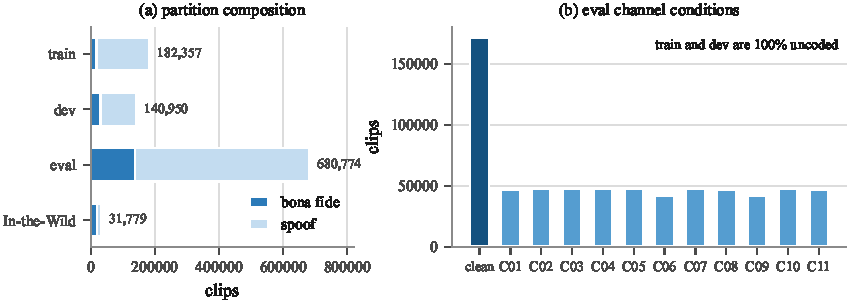
\includegraphics[width=\columnwidth]{figures/fig10_dataset}
\caption{(a)~Partition composition. (b)~Channel conditions of the evaluation
set. The development split has none of the eleven coded conditions on which
the evaluation set is judged.}
\label{fig:dataset}
\end{figure}

% =========================================================================
\section{Systems}
\label{sec:systems}

\subsection{Shared Pipeline}

\begin{figure}[t]
\centering
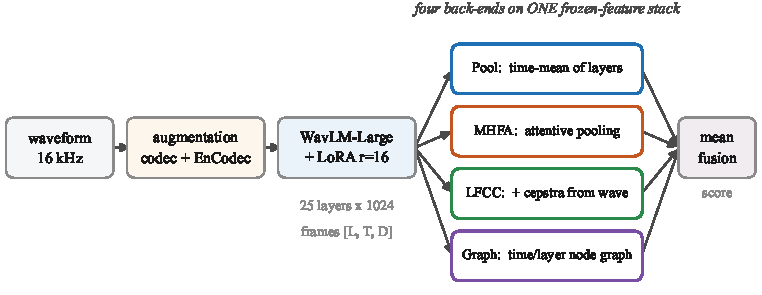
\includegraphics[width=\columnwidth]{figures/fig1_architecture}
\caption{Shared pipeline. The four members use the same waveform path, the same
augmentation and the same adapted WavLM-Large backbone. They differ only in
the back-end that turns per-layer frames into a score.}
\label{fig:arch}
\end{figure}

Fig.~\ref{fig:arch} shows the pipeline. A waveform is augmented, then passed
through WavLM-Large~\cite{wavlm} adapted with LoRA~\cite{lora} of rank 16 on
the attention projections. That gives 3.15M trainable parameters out of 315M.
The backbone returns 25 layer activations. During training, one of eight
simulated codecs is applied with probability 0.5. EnCodec~\cite{encodec} is
applied on the GPU with probability 0.3. EnCodec stands in for the neural
codecs of evaluation conditions C04 and C07.

Members are combined by the unweighted mean of their scores, each standardised
on the development \texttt{calib} split. No parameter of the combiner is fit
on evaluation data.

\begin{table}[t]
\centering
\caption{Training settings shared by all members.}
\label{tab:recipe}
\small
\begin{tabular}{ll}
\toprule
Setting & Value \\
\midrule
Main backbone & WavLM-Large \\
Second backbone & XLS-R-300M \\
Adapter & LoRA, rank 16 \\
Head learning rate & $10^{-3}$ \\
Backbone learning rate & $10^{-5}$ \\
Batch size & 32 \\
Epochs & 8 \\
Seed & 1337 \\
Classical codec probability & 0.5 \\
EnCodec probability & 0.3 \\
\bottomrule
\end{tabular}
\end{table}

\subsection{The Four Back-Ends}

\textit{Pool} has 0.26M parameters. It takes the time-mean of each layer,
learns a softmax weighting over the layers and applies a two-layer MLP. This is
the conventional design, and it throws the time axis away at the first step.

\textit{MHFA} has 0.53M parameters. It keeps the frames. Following Peng and
colleagues~\cite{mhfa}, it learns two separate layer weightings, one for keys
and one for values, and pools over time with multi-head attention.

\textit{LFCC} has 0.50M parameters. It adds a second representation: 20
linear-frequency cepstral coefficients with first and second differences,
computed from the waveform and aligned frame by frame with the backbone. They
are concatenated with the backbone features before attentive
pooling~\cite{attentive_pool}. Part of the evidence this branch sees cannot
correlate with anything the backbone encodes.

\textit{Graph} has 0.30M parameters. It adds a second topology, with graph
attention over two sets of nodes: time slots and backbone layers. It reuses
the graph attention layer of AASIST~\cite{aasist}. It has no heterogeneous
cross-attention and no master node, so it is not AASIST.

\subsection{Measuring Independence}
\label{sec:metrics}

Let $\mathbf{R}$ be the correlation matrix of the $M$ members' evaluation
scores, with eigenvalues $\lambda_i$. We summarise it with the participation
ratio and the entropy rank,
\begin{align}
\PR &= \frac{\bigl(\sum_i \lambda_i\bigr)^2}{\sum_i \lambda_i^2},
\label{eq:pr}\\
\HR &= \exp\!\Bigl(-\sum_i p_i \log p_i\Bigr),\quad
  p_i = \frac{\lambda_i}{\sum_j \lambda_j}.
\label{eq:hr}
\end{align}
Both equal 1 when all members are identical and $M$ when they are fully
uncorrelated.

Two properties make these numbers easy to use. Both are unchanged if every
score is rescaled or shifted, because the correlation matrix ignores scale.
Both also run from 1 to $M$ and reach $M$ only when the eigenvalues are all
equal. The participation ratio is the exponential of the order-2 R\'enyi
entropy of $p$, and the entropy rank is the exponential of its Shannon
entropy. The first is dominated by the largest eigenvalue. The second gives
more weight to the small ones, so it reads higher when a few weak directions
carry independent signal. We report both for that reason.

A quick check shows how the headline number arises. With $M{=}4$ the
eigenvalues sum to 4. If the first component explains 95.5\% of the variance,
then $\lambda_1 \approx 3.82$ and the other three sum to about 0.18. The
square of $\lambda_1$ is about 14.6, the other squares add almost nothing, and
so the ratio is $16/14.6 \approx 1.10$. The reported value follows directly
from the 95.5\% figure.

% =========================================================================
\section{Protocol}
\label{sec:protocol}

We choose models on the development \texttt{select} split (attacks A09 to
A16). Score statistics are fit on the speaker-disjoint \texttt{calib} half.
The evaluation set is scored once. We report \eer{}, \mindcf{} under the
official ASVspoof~5 cost model (spoof prior 0.05, miss cost 1, false-alarm
cost 10)~\cite{asvspoof5,tdcf}, and the minimum log-likelihood-ratio cost.
Differences between systems use a paired bootstrap that resamples source
utterances.

Every member uses seed 1337 and the settings in Table~\ref{tab:recipe}.
\textbf{Every number below comes from one seed.} In earlier experiments on this
codebase, three seeds of a frozen single model spread over 0.33 \eer{} points.
That is more than three times the 0.10-point gain we report for fusion. So we
do not know the seed variance of the systems in Table~\ref{tab:members}, and
the fusion gain should be read with that in mind.

% =========================================================================
\section{Results}
\label{sec:results}

\subsection{The Four Members}

\begin{table*}[t]
\centering
\caption{The four members. They share everything except the back-end. Dev sel.\
is the mean \eer{} over the clean and codec development views. The last column
is the Pearson correlation of evaluation scores with Pool. Lower is better for
all error columns. Bold marks the best value in a column.}
\label{tab:members}
\small
\begin{tabular}{llrrrrrr}
\toprule
& & & \multicolumn{3}{c}{ASVspoof~5 eval} &
  \multicolumn{1}{c}{In-the-Wild} & \\
\cmidrule(lr){4-6}\cmidrule(lr){7-7}
Member & Differs in & Dev sel. &
  \eer{} & \mindcf{} & min$C_\text{llr}$ & \eer{} & $\rho_{\text{Pool}}$ \\
\midrule
Pool  & baseline        & \best{1.50} & 3.31 & 0.0942 & 0.1256 & 11.25 & n/a \\
MHFA  & pooling         & 2.07 & 3.44 & 0.0957 & 0.1286 & \best{8.51} & 0.917 \\
LFCC  & representation  & 2.95 & \best{3.11} & \best{0.0845} & \best{0.1164} & 11.82 & 0.965 \\
Graph & topology        & 3.10 & 3.93 & 0.1091 & 0.1475 & 11.44 & 0.943 \\
\bottomrule
\end{tabular}
\end{table*}

Table~\ref{tab:members} is the central table, and almost every column
disagrees with every other. Pool is best on development and only third on
evaluation. LFCC is worst on development, best on evaluation, and worst again
on found audio. MHFA is third in domain at 3.44\% and first out of domain at
8.51\%, a 24\% relative lead over the next system.

The last column matters most for the rest of the paper. Every member
correlates with Pool at 0.917 or higher. MHFA, the member that keeps the time
axis, is the least correlated. Fig.~\ref{fig:curves} shows that these
differences are not artefacts of training.

\begin{figure}[t]
\centering
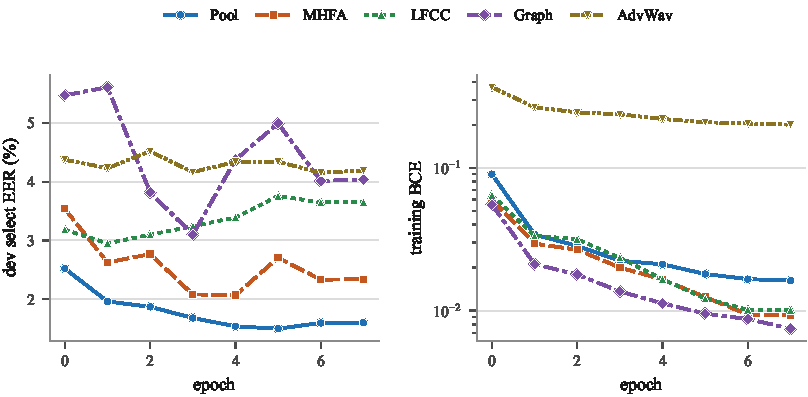
\includegraphics[width=\columnwidth]{figures/fig2_training_curves}
\caption{Training behaviour. Left: development \eer{}. Right: training loss.
The adversarially trained system of Section~\ref{sec:robust} converges to
roughly double the development \eer{} of every other member.}
\label{fig:curves}
\end{figure}

\subsection{Comparison with Published Systems}

\begin{table}[t]
\centering
\caption{Comparison with published ASVspoof~5 open-condition results. Lower is
better. $^\dagger$Oracle subset, shown for reference only
(Section~\ref{sec:selection}).}
\label{tab:comparison}
\small
\begin{tabular}{lrr}
\toprule
System & \eer{} & \mindcf{} \\
\midrule
USTC-KXDIGIT~\cite{ustc2024}, 12 fused & 2.59 & 0.0750 \\
SZU-AFS~\cite{szuafs}, single system & 4.04 & 0.1150 \\
\midrule
This work, Pool (single) & 3.31 & 0.0942 \\
\best{This work, Pool + MHFA (selected)} & \best{3.21} & \best{0.0905} \\
This work, Pool + LFCC$^\dagger$ & \textit{2.93} & \textit{0.0819} \\
\bottomrule
\end{tabular}
\end{table}

Table~\ref{tab:comparison} places the results next to the two systems we
compare against, both taken from their published reports. Our selected system
is 20\% better in relative \eer{} than SZU-AFS. It is behind the twelve-system
winner by 0.62 points. Our own single Pool model already beats SZU-AFS, so the
fusion gain starts from a good base. We train on ASVspoof~5 only, and the
winner trains on more data, so the comparison does not isolate the effect of
architecture.

\subsection{Conditions and Attacks}

Fig.~\ref{fig:codec} splits the evaluation set by channel. The two neural
codecs, C04 and C07, are the hardest conditions for every member by a wide
margin. They were even harder before we added EnCodec to training. Attack A28
alone gives an \eer{} of 9.36\%, while nine of the sixteen evaluation attacks
sit below 1.5\%. The pooled number therefore says a lot about one attack. The
attacker-adaptation conditions are flat, at 3.29\%, 3.14\% and 3.19\% for AC1,
AC2 and AC3, so adaptation strength made no difference we could measure.

\begin{figure}[t]
\centering
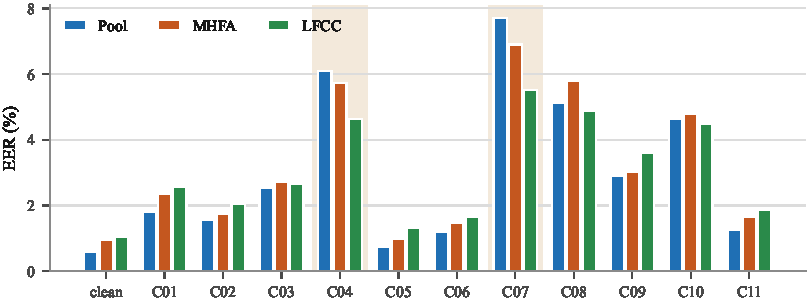
\includegraphics[width=\columnwidth]{figures/fig4_per_codec}
\caption{\eer{} by channel condition. The neural codecs C04 and C07 are the
hardest conditions for every member, and the development split contains
neither.}
\label{fig:codec}
\end{figure}

\subsection{How Many Independent Systems?}
\label{sec:rank}

\begin{figure*}[t]
\centering
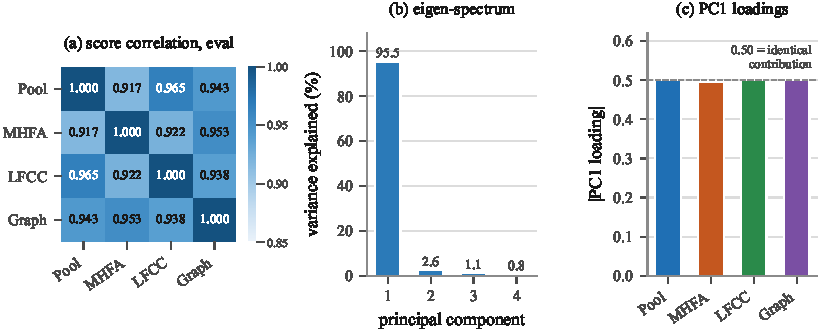
\includegraphics[width=\textwidth]{figures/fig6_spectrum}
\caption{(a)~Score correlation on the evaluation set. (b)~Eigenvalue spectrum
of that matrix: the first component explains 95.5\% of the variance.
(c)~Loadings of the first component are within 0.006 of 0.50 on every member,
so the component is the unweighted mean.}
\label{fig:spectrum}
\end{figure*}

Fig.~\ref{fig:spectrum} gives the answer, using the definitions of Section~\ref{sec:metrics}. The participation ratio is 1.10 out
of four, and the entropy rank is 1.26. The first component explains 95.5\% of
the variance, with loadings of 0.501, 0.496, 0.501 and 0.502. On the
out-of-domain set the figure is 1.15 out of four. Changing pooling,
representation, topology and backbone moves the effective rank by only 0.1.

This changes how we should read fusion results. The best two-member fusion
(Pool and LFCC) improves on its best single member by 0.18 \eer{} points, and
a third member adds nothing. The USTC-KXDIGIT system gains 35\% relative from
twelve systems across three back-end families~\cite{ustc2024}, and that gain
needs the kind of diversity our members lack. The only change that moved our
correlation was a change in what the model sees. Replacing time-mean pooling
with frame attention took the correlation from 0.994 to 0.917.

\subsection{Why Selection Fails}
\label{sec:selection}

\begin{table*}[t]
\centering
\caption{Member subsets ranked by development \eer{}: the top four of fifteen,
plus the best subset on evaluation. Our protocol takes rank 1. The oracle row
is for comparison only and is not claimed as a result.}
\label{tab:selection}
\small
\begin{tabular}{llrrrr}
\toprule
Rank & Subset & Dev sel. & eval \eer{} & eval \mindcf{} & ITW \eer{} \\
\midrule
\multicolumn{6}{l}{\textit{Clean + codec development views (rank correlation $+0.011$, $p{=}0.97$)}}\\
1 & Pool + MHFA          & \best{1.46} & 3.21 & 0.0905 & 9.04 \\
2 & Pool                 & 1.47 & 3.31 & 0.0942 & 11.25 \\
3 & Pool + MHFA + Graph  & 1.67 & 3.20 & 0.0903 & 8.80 \\
4 & Pool + MHFA + LFCC   & 1.72 & 2.94 & 0.0827 & 9.04 \\
7 & \textit{Pool + LFCC (oracle)} & 1.83 & \textit{2.93} & \textit{0.0819} & 9.19 \\
\midrule
\multicolumn{6}{l}{\textit{Neural-codec view added (rank correlation $+0.236$, $p{=}0.40$)}}\\
1 & Pool + MHFA          & \best{2.79} & 3.21 & 0.0905 & 9.04 \\
2 & Pool + MHFA + LFCC   & 2.90 & 2.94 & 0.0827 & 9.04 \\
6 & \textit{Pool + LFCC (oracle)} & 3.01 & \textit{2.93} & \textit{0.0819} & 9.19 \\
\bottomrule
\end{tabular}
\end{table*}

\begin{figure}[t]
\centering
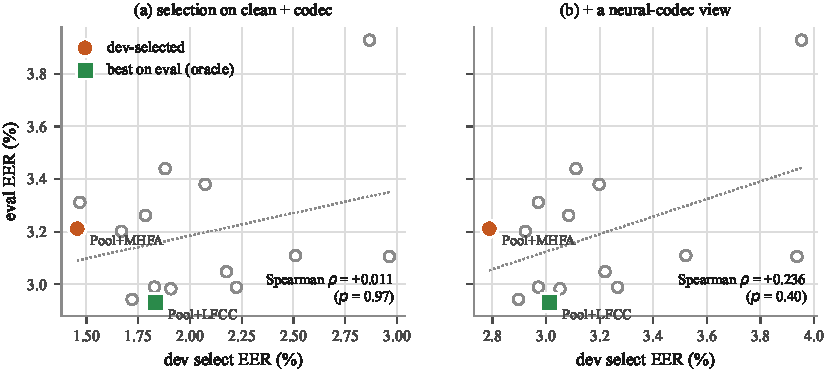
\includegraphics[width=\columnwidth]{figures/fig7_selection}
\caption{Development \eer{} against evaluation \eer{} for all 15 member
subsets. The neural-codec view improves the ordering, and one subset climbs
from rank 4 to rank 2, but selection is still not predictive.}
\label{fig:selection}
\end{figure}

Over all 15 subsets the rank correlation between development and evaluation
error is $+0.011$ ($p{=}0.97$). The development split says nothing about the
evaluation order (Fig.~\ref{fig:selection}). The reason is plain. The
conditions that separate systems on evaluation are real codecs, and the
development split has none of them.

We tried to repair this by adding a neural-codec development view. The
correlation rises to $+0.236$, and one subset climbs from rank 4 to rank 2.
That is real progress, but at $p{=}0.40$ it is still indistinguishable from
zero.

Our protocol selects Pool and MHFA, at \textbf{3.21\% \eer{} and 0.0905
\mindcf{}}. The oracle is Pool and LFCC at 2.93\% and 0.0819, which the
protocol ranks seventh of fifteen. We report both numbers and read the 0.28
point gap as a measurement of how much the selection set is worth, not as a
result we can claim.

\subsection{Domain Transfer}

\begin{figure}[t]
\centering
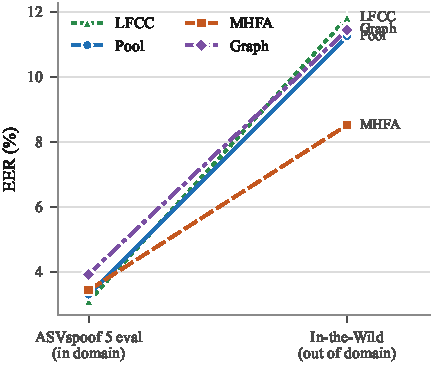
\includegraphics[width=\columnwidth]{figures/fig8_transfer}
\caption{In-domain and out-of-domain \eer{}. Every system degrades by a factor
of 2.5 to 3.8 on In-the-Wild, and the ordering flips.}
\label{fig:transfer}
\end{figure}

Fig.~\ref{fig:transfer} shows the factor of 2.5 to 3.8 that M\"{u}ller and
colleagues~\cite{intothewild} also report for lab-trained detectors. The flip
in order is the new part. LFCC is our best in-domain member at 3.11\% and our
worst on found audio at 11.82\%. MHFA goes from third (3.44\%) to first
(8.51\%).

One possible reading is that cepstral features partly capture recording
conditions, which do not carry over from a curated corpus to audio found
online, while frame-level attention learns something less tied to the corpus.
We offer this as a guess. Our experiments show the flip but do not explain it.
The practical point stands either way. Chasing the last 0.6 \eer{} points
in domain would mean picking the member that transfers worst.

\begin{figure}[t]
\centering
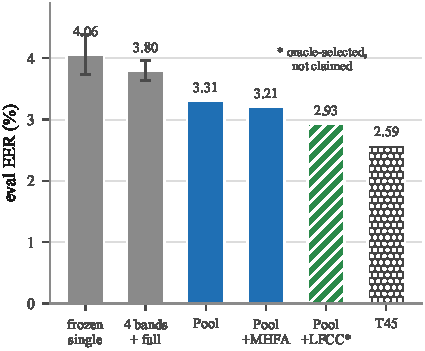
\includegraphics[width=\columnwidth]{figures/fig9_progress}
\caption{Progress of this work. Bars with error bars are three-seed means. The
hatched bar is the oracle-selected subset.}
\label{fig:progress}
\end{figure}

% =========================================================================
\section{Adversarial Robustness}
\label{sec:robust}

\begin{table*}[t]
\centering
\caption{Attack success rate at a 0.1\% false-alarm operating point. PGD
uses 20 steps under an SNR-constrained $L_2$ budget~\cite{madry2018}, and the
realised SNR is reported. SPSA is a black-box attack with 320 queries per clip.
The table is generated from the attack logs, so it cannot drift from the
measurements. Four defence routes are closed. Waveform adversarial training is
the only one that moves white-box success off 1.000.}
\label{tab:robust}
\small
% generated by paper/robustness_table.py -- do not edit by hand
\begin{tabular}{llrrr}
\toprule
Defence & Attack & Clean \eer{} & 30\,dB & 20\,dB \\
\midrule
single model & white-box PGD & 4.78 & 1.000 & 1.000 \\
single model & SPSA & 4.78 & --- & 0.011 \\
four layer bands & white-box PGD & 4.78 & 1.000 & 1.000 \\
four layer bands & transfer PGD & 4.78 & 1.000 & 1.000 \\
four layer bands & SPSA & 4.78 & --- & 0.014 \\
WavLM, surrogate XLS-R & white-box PGD & 4.78 & 1.000 & 1.000 \\
WavLM, surrogate XLS-R & transfer PGD & 4.78 & 0.892 & 0.995 \\
XLS-R, surrogate WavLM & white-box PGD & 9.21 & 1.000 & 1.000 \\
XLS-R, surrogate WavLM & transfer PGD & 9.21 & 0.832 & 0.984 \\
feature-space adv.\ training & white-box PGD & 13.95 & 0.993 & 1.000 \\
feature-space adv.\ training & transfer PGD & 13.95 & 0.776 & 0.977 \\
\textbf{waveform adv.\ training} & white-box PGD & 7.07 & 0.953 & 0.967 \\
\textbf{waveform adv.\ training} & transfer PGD & 7.07 & 0.739 & 0.951 \\
its control (Pool) & white-box PGD & 4.17 & 1.000 & 1.000 \\
its control (Pool) & transfer PGD & 4.17 & 1.000 & 1.000 \\
\bottomrule
\end{tabular}

\end{table*}

\subsection{Threat Model}

We consider three attackers. The white-box attacker has the gradient of the
score with respect to the waveform and runs 20 steps of PGD. The transfer
attacker has the gradient of a surrogate model, for example XLS-R when the
target is WavLM, and applies the result to the target. The black-box attacker
can only query the score and uses SPSA with 320 queries per clip. In all
cases the perturbation is limited by signal-to-noise ratio, at 30\,dB and at
20\,dB, and success means that a spoofed clip is scored as bona fide at the
operating point where the false-alarm rate is 0.1\%. The realised SNR is
measured and reported, not assumed.

\subsection{Findings}

Table~\ref{tab:robust} lists the measurements. An attacker with gradients
succeeds on almost every clip at 30\,dB SNR against four of the five defences.
Those four are a single model, a four-member ensemble of layer bands, each of
two SSL backbones attacked through the other as a surrogate, and feature-space
adversarial training. The last one also ruined clean accuracy, with an \eer{}
of 13.95\%. An attacker who can only query the model, with 320 queries per
clip, succeeds on about 1\% of clips.

Waveform adversarial training is the one route that moves. Half of each
training batch is replaced by 30\,dB PGD examples crafted through the
backbone, which hardens the path an attacker actually takes. White-box success
falls from 1.000 to 0.953 at 30\,dB, and transfer success falls from 1.000 to
0.739. Its control, trained the same way without the adversarial half, stays
at 1.000 on every row. So the drop comes from the defence and not from the
training schedule.

The cost is large. Clean \eer{} rises from 3.31\% to 7.09\%, a paired
difference of $+0.0378$ with a 95\% interval of $[+0.0372,\,+0.0384]$ over all
680{,}774 clips. The codec conditions suffer most (C07 at 11.06\%, C08 at
10.08\%). Five points off the attack success rate for 3.78 points of clean
error is not a trade a deployed system would take. A detector that still falls
to nineteen attacks in twenty is not protected.

The feature-space result needs a caveat. That defence hardened the head
against perturbations in feature space, while the attacker perturbs the
waveform and reaches the head through the backbone. Because of this mismatch,
its failure is weak evidence. The waveform run is the corrected experiment.
It recovered 6.9 points of clean accuracy relative to the feature-space
attempt, and it was the only change that moved white-box success at all.

% =========================================================================
\section{Discussion}
\label{sec:discussion}

\subsection{Why Variety in Architecture Is Not Enough}

The intuition behind fusion is that systems built differently fail
differently. Our data say this is false when the systems share a backbone. All
four members read the same backbone features, and those features are dominated
by signal that is common to every layer and every codec. A different pooling
rule, a graph on top, or a second branch changes where the decision boundary
sits. It does not change the evidence the boundary is drawn through. Systems
that draw different boundaries through the same evidence still agree on most
utterances.

This account also explains the exception. MHFA keeps the time axis, so it can
see a vocoder artefact confined to a short stretch of frames. Pool has averaged
that stretch away before it makes any decision. MHFA is the least correlated
member with Pool, at 0.917. For anyone building a shared-backbone ensemble the
advice is practical. Give the members access to different information, and do
not expect a different architecture on the same information to help.

\subsection{What to Do With the Participation Ratio}

The participation ratio can be computed before the expensive part. Score a
candidate pool on held-out data, form the correlation matrix, and see whether a
new member raises the ratio. If it does not, the member is not adding
independent evidence, and training it further is unlikely to pay. We have not
tested a numeric threshold for this decision. That would need many more
ensembles than the one we studied.

\subsection{Selection on ASVspoof 5}

The 0.28 point gap between our selected system and the oracle is small in
absolute terms. It still matters for method. Any ablation or architecture
search that looks only at the uncoded development split of ASVspoof~5 is
choosing with a signal we measured at $+0.011$. Reported rankings of
systems on this benchmark, including ours, deserve a second look for this
reason.

\subsection{Robustness as a Measurement}

We present the robustness results as measurements. Papers often say that a
defence improves robustness without stating what it costs on clean data at the
same operating point. Here the only defence that moves the white-box frontier
also roughly doubles the clean error, from 3.31\% to 7.09\%. Whether that is
acceptable depends on the threat model. For most deployments it is not, and we
do not claim that the frontier cannot be pushed further.

% =========================================================================
\section{Limitations}
\label{sec:limit}

\textbf{One seed.} Every system in Table~\ref{tab:members} is one run. Earlier
three-seed runs gave a 0.33-point spread on frozen single models, which is
larger than the 0.10-point fusion gain. The fusion gain is therefore not
established against seed variance. Repeating Pool and MHFA over several seeds
is the most important missing experiment.

\textbf{One training corpus.} We train on ASVspoof~5 alone, and the USTC system~\cite{ustc2024}
trains on four corpora. We cannot separate a weaker architecture from narrower
supervision.

\textbf{Interval width.} Clip-level bootstrap intervals on this corpus are
about twice too narrow. Our own conclusions survive the correction because the
differences are many standard errors wide, but intervals reported elsewhere on
this corpus may not.

\textbf{One out-of-domain set.} In-the-Wild has its own biases. It holds public
figures and internet audio, and its class balance is reversed. One such set
measures a gap. It does not describe generalisation in general.

\textbf{No ablations of the training recipe.} We did not ablate the codec
simulation, the adapter rank or the layer weighting, so we cannot say how much
each contributes. We also did not compare the participation ratio with pairwise
diversity measures.

\textbf{The Graph member is not AASIST.} No result here should be cited as
evidence about AASIST~\cite{aasist}.

\subsection{What We Would Do Next}

Three experiments would make the claims firmer. The first is to train Pool and
MHFA over several seeds, so that the 0.10-point fusion gain can be compared
with a measured seed spread and not with an earlier one from a different
setting. The second is to give the members different evidence on purpose, for
example a second backbone trained on a different corpus, and to check whether
the participation ratio rises. Our fifth system changed the backbone and moved
the rank by only 0.1, but it was trained on the same data. The third is to
ablate the codec simulation, which we believe is responsible for the change
in the neural-codec conditions but have not isolated.

% =========================================================================
\section{Conclusion}
\label{sec:conclusion}

Four detectors that differ in pooling, representation, topology and backbone
behave like 1.10 independent systems. Variety in architecture is not variety
in errors. The one change that moved the correlation was a change in what the
model sees.

The corpus that most of the field uses for selection could not rank these
systems, and the choice it made cost 0.28 \eer{} points against our own
oracle. The best member in domain was the worst on found audio. The only
defence that lowered white-box attack success also doubled the clean error.

Our selected system reaches \textbf{3.21\% \eer{} and 0.0905 \mindcf{}}. That is
ahead of SZU-AFS at 4.04\% and 0.115~\cite{szuafs}, and behind the
twelve-system winner at 2.59\% and 0.0750~\cite{ustc2024}. We think the
measurements around that number are worth more than the number. They give a
way to count how many systems an ensemble really holds, and they show that the
standard selection step on this benchmark does not work.

\subsubsection*{Reproducibility.}
Figures are produced by \texttt{paper/make\_figures.py} from one JSON file of
measured values, so no number in the text can disagree with a figure. The
robustness table is generated from the attack logs. Every experiment,
including the failures, is recorded in \texttt{docs/experiment\_log.md}.

% =========================================================================
\bibliographystyle{unsrt}
\bibliography{refs}

\end{document}
